%---
\section{RADIOACTIVE SOURCE CALIBRATION OF DARKSIDE-50}
\label{sec:calibration}

During 2014, calibration hardware to deploy radioactive sealed sources within the LSV was developed by DarkSide collaborators. CALIS (CALibration Insertion System) is designed to deploy radioactive sources to calibrate both the LAr-TPC and the LSV. CALIS has been constructed, tested at Fermilab and LNGS, precision cleaned, and successfully installed in the DarkSide clean room (Fig.~\ref{fig:CALIS}, left). 

\begin{figure}[htbp]
\centering
\subfigure{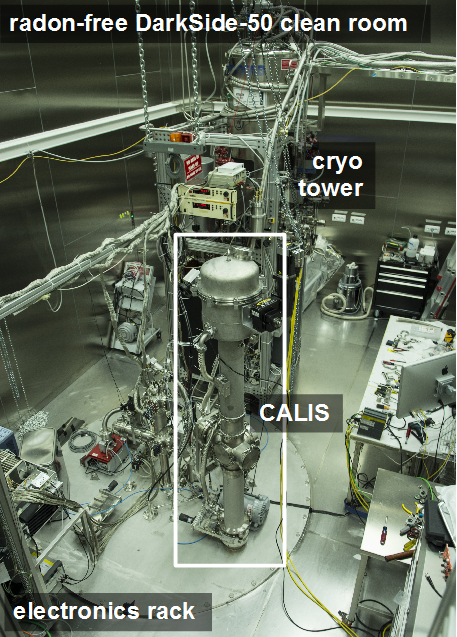
\includegraphics[width=0.4\textwidth]{./Figures/CALISinCRH.png}}
\subfigure{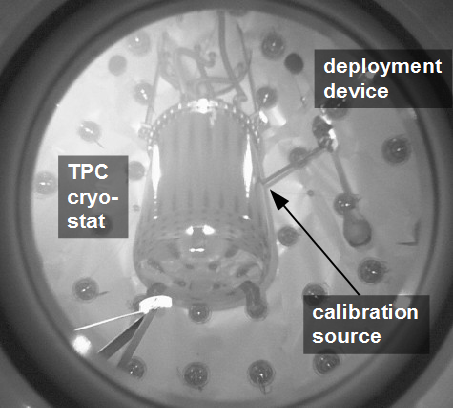
\includegraphics[width=0.47\textwidth]{./Figures/Next2Cryostat.png}}
\caption{\textit{left}: CALIS after installation inside the CRH radon-suppressed clean room atop the WCD. \textit{right}: Photograph taken with a camera looking into the LSV from the WCD. It  shows a source deployed next to the cryostat of the LAr-TPC.
\label{fig:CALIS}}
\end{figure}

%\subsection{Source Deployment}
\noindent \textbf{Source Deployment}: In order to deploy a radioactive source next to the LAr-TPC, the source is brought into the CRH radon-suppressed clean room atop the WCD tank, and mounted in a source holder connected to the deployment device within CALIS. This is lowered into the LSV through a dedicated access port, to a position next to the cryostat. The source holder is on the end of a 60 cm long articulated arm, which can be moved and rotated to position the source in 3-D relative to the cryostat (Fig.~\ref{fig:CALIS}, right). Throughout the deployment a slightly pressurized nitrogen atmosphere has to be maintained in order to avoid exposing the liquid scintillator to oxygen or water, which would degrade it. All materials used for CALIS, such as stainless steel, teflon, and viton, that come in contact with the scintillator are certified for contact with the liquid scintillator. The system includes several safety features to ensure safe deployment and retrieval of the source without affecting the stability and performance of the LSV. After data taking, the deployment device is retracted and a sequence of N$_2$ purging and evacuation removes all traces of scintillator from the deployment device. Thereafter the source holder can be extracted from the deployment device and the radioactive source returned to storage.
The CALIS concept has the built-in flexibility to deploy different devices next to the cryostat, e.g.~the deployment of a (d,d) neutron generator is considered in the future.

%\subsection{Calibration Campaign}
\noindent \textbf{Calibration Campaigns:} After the calibration device and the deployment procedures were approved by the DarkSide scientific committee, two extensive calibration campaigns were performed during October through December 2014 and January through February 2015. The performance and stability of the LSV and LAr-TPC was not affected by the two calibration campaigns.

Since these were the first \dsf\ calibration campaigns using external radioactive sources, a broad range of physics topics was addressed by deploying three gamma sources with different energies ($^{57}$Co, $^{133}$Ba and $^{137}$Cs) and two AmBe neutron sources. The AmBe neutron source deployments allowed us to make the first in-situ measurements of the \dsf\ system's responses to neutrons both in the LAr-TPC and the LSV.
Systematic studies were made of the effects of varying detector conditions such as the drift field (null field, 100 V/cm, 150 V/cm, 200 V/cm) and varying source positions relative to the TPC. These studies are furthering our understanding of the detector and allow accurate tuning of the detector optics and LAr microphysics embodied in G4DS, our DarkSide-50 Monte Carlo. 